\chapter{البوليمرات: التخليق والبنية والخصائص}\label{ch:b2:polymer-synthesis}

طُرحت جوارب النايلون للبيع سنة 1939. وقد خرجت من مختبر شرع، قبل ذلك ببضع
سنوات، في فهم كيف تتحد الجزيئات الصغيرة في جزيئات طويلة، وتعلّم في الطريق
درسًا يفاجئ كل كيميائي أول مرة: فمن أجل \omterm{def:b2:polymer-synthesis:polymer}{بوليمر} يُصنع بوصل الجزيئات طرفًا بطرف،
لا يكفي مردود 99~\%. ويفسر هذا الفصل السبب، ويصف الطريقتين اللتين تنمو بهما السلاسل،
ويربط بنية السلاسل بخصائص المواد.
% ledger: hist:nylon-production-1939

\begin{recall}
المجلد المدرسي: البوليمرات، \omterm{def:b2:polymer-synthesis:polymer}{والمونومرات} والوحدات المتكررة، وبوليمرات الإضافة والتكاثف،
واللدائن الحرارية والمتصلدة بالحرارة. ومجلد السنة الأولى: الجذور والانشطار المتجانس، والكاتيونات الكربونية 
والأنيونات الكربونية، وتقريب الحالة المستقرة. و\cref{ch:b2:acyl-substitution}: الإسترات والأميدات.
و\cref{ch:b2:catalytic-cycles}: الإدخال في رابطة فلز--كربون.
\end{recall}

\section{السلاسل وكتلها المولية}

\begin{definition}[البوليمر]\label{def:b2:polymer-synthesis:polymer}
\emph{البوليمر}\index{بوليمر} مادة مكوّنة من جزيئات ضخمة، يُبنى كل منها بالوصل المتكرر
لجزيئات صغيرة، هي \emph{المونومرات}\index{مونومر}. و\emph{الوحدة المتكررة}\index{وحدة متكررة}
هي أصغر مجموعة من الذرات يُكوّن تكرارها السلسلة؛ و\emph{درجة
البلمرة}\index{درجة البلمرة} $X$ لسلسلة هي عدد الوحدات المشتقة من المونومرات
التي تحويها.
\end{definition}

عينة \omterm{def:b2:polymer-synthesis:polymer}{البوليمر} الصنعي لا تتكوّن أبدًا من سلاسل متطابقة: فهي خليط من سلاسل
مختلفة الأطوال، وكتلتها المولية متوسط يتعلق بطريقة عدّ السلاسل.

\begin{definition}[متوسطات الكتلة المولية]\label{def:b2:polymer-synthesis:averages}
من أجل عينة تحوي $N_i$ سلسلة كتلتها المولية $M_i$، تكون \emph{الكتلة المولية المتوسطة
العددية}\index{كتلة مولية متوسطة عددية} و\emph{الكتلة المولية المتوسطة الكتلية}\index{كتلة مولية متوسطة كتلية}
هما
\begin{equation*}
\bar M_n = \frac{\sum_i N_i M_i}{\sum_i N_i}, \qquad
\bar M_w = \frac{\sum_i N_i M_i^2}{\sum_i N_i M_i} = \sum_i w_i M_i,
\end{equation*}
حيث $w_i$ الكسر الكتلي للسلاسل ذات الكتلة $M_i$. و\emph{التشتت}\index{تشتت}
$\text{\DH} = \bar M_w/\bar M_n$ لا يقل عن 1، ولا يساوي 1 إلا إذا كان لكل السلاسل
الكتلة نفسها. ويُعرَّف المتوسطان $\bar X_n$ و$\bar X_w$ \omterm{def:b2:polymer-synthesis:polymer}{لدرجة البلمرة} بالطريقة
نفسها.
\end{definition}

المتوسط العددي يزن كل سلسلة مرة واحدة؛ والمتوسط الكتلي يزن كل سلسلة بكتلتها، فتكون
للسلاسل الطويلة وزن أكبر. وكون $\text{\DH} \ge 1$ هو المتباينة $\left(\sum N_i M_i\right)^2 \le
\sum N_i \sum N_i M_i^2$ (كوشي--شفارتز)، ولا تتحقق المساواة إلا عند تساوي $M_i$.

\begin{method}[حساب المتوسطات]\label{met:b2:polymer-synthesis:averages}
\begin{enumerate}
  \item حوّل المعطيات إلى كميات $N_i$ (أو أعداد سلاسل) وكتل $M_i$؛ وانطلاقًا من الكسور الكتلية،
        $N_i \propto w_i/M_i$.
  \item $\bar M_n = \sum N_i M_i / \sum N_i$؛ أو بعبارة مكافئة، $1/\bar M_n = \sum w_i/M_i$.
  \item $\bar M_w = \sum w_i M_i$.
  \item $\text{\DH} = \bar M_w/\bar M_n$؛ وتحقق من أن $\bar M_w \ge \bar M_n$.
\end{enumerate}
\end{method}

\section{النمو المرحلي والنمو السلسلي}

\begin{definition}[النمو المرحلي والنمو السلسلي]\label{def:b2:polymer-synthesis:step-chain}
في \emph{البلمرة بالنمو المرحلي}\index{بلمرة بالنمو المرحلي}، يمكن لأي جزيئين يحملان
مجموعتين وظيفيتين متكاملتين (مونومرات، أو أوليغومرات أو سلاسل طويلة) أن يتفاعلا، وتطول
السلاسل باتصال بعضها ببعض: البوليسترات والبوليأميدات. وفي \emph{البلمرة بالنمو
السلسلي}\index{بلمرة بالنمو السلسلي}، يضيف مركز تفاعلي (جذر، أو أيون أو رابطة فلز--كربون)
جزيئات \omterm{def:b2:polymer-synthesis:polymer}{المونومر} واحدًا تلو الآخر إلى طرف سلسلة نامية: بوليمرات الألكينات.
\end{definition}

\begin{method}[مرحلي أم سلسلي؟]\label{met:b2:polymer-synthesis:classify}
\begin{enumerate}
  \item \omterm{def:b2:polymer-synthesis:polymer}{مونومر} ذو مجموعتين وظيفيتين تتفاعل كل منهما مع شريكة الأخرى (حمض وكحول،
        حمض وأمين)، وغالبًا ما يتحرر جزيء صغير: نمو مرحلي.
  \item \omterm{def:b2:polymer-synthesis:polymer}{مونومر} ذو رابطة مزدوجة \ce{C=C} (أو حلقة متوترة) وبادئ: نمو سلسلي.
  \item تحقق بمسار التفاعل: في النمو المرحلي يختفي \omterm{def:b2:polymer-synthesis:polymer}{المونومر} مبكرًا ولا تظهر السلاسل الطويلة
        إلا في النهاية تمامًا؛ وفي النمو السلسلي تظهر السلاسل الطويلة منذ البداية بينما يُستهلك \omterm{def:b2:polymer-synthesis:polymer}{المونومر}
        تدريجيًا.
\end{enumerate}
\end{method}

\subsection*{النمو المرحلي}

لنأخذ خليطًا متوازنًا من مونومرات \ce{A-A} و\ce{B-B} (ثنائي أمين وثنائي حمض)، أو مونومرًا واحدًا
\ce{A-B}. ولنسمِّ $p$ \emph{درجة تقدم التفاعل}: أي كسر المجموعات الوظيفية من أحد
النوعين التي تفاعلت.

\begin{theorem}[معادلة كاروثرز]\label{thm:b2:polymer-synthesis:carothers}
في \omterm{def:b2:polymer-synthesis:step-chain}{بلمرة بالنمو المرحلي} لمونومرات ثنائية الوظيفة متوازنة تمامًا، تكون \omterm{def:b2:polymer-synthesis:polymer}{درجة
البلمرة} المتوسطة العددية، معدودة بوحدات \omterm{def:b2:polymer-synthesis:polymer}{المونومر}،
\begin{equation*}
\bar X_n = \frac{1}{1 - p}.
\end{equation*}
\end{theorem}

\begin{proof}
لنبدأ بعدد $N_0$ من جزيئات \omterm{def:b2:polymer-synthesis:polymer}{المونومر}، تحمل $N_0$ مجموعة \ce{A} و$N_0$ مجموعة \ce{B}. كل تفاعل
بين \ce{A} و\ce{B} يصل جزيئين في جزيء واحد، فيخفض عدد الجزيئات بمقدار
واحد. وبعد $pN_0$ تفاعلًا يبقى $N = N_0 - pN_0 = N_0(1-p)$ جزيئًا تتقاسم وحدات \omterm{def:b2:polymer-synthesis:polymer}{المونومر} البالغ عددها
$N_0$: $\bar X_n = N_0/N = 1/(1-p)$.
\end{proof}

\begin{corollary}[عدم التوازن]\label{cor:b2:polymer-synthesis:imbalance}
إذا لم تكن المجموعات متوازنة، مع $r = N_{\ce{A}}/N_{\ce{B}} \le 1$ و$p$ درجة تقدم تفاعل
المجموعات الأقلية \ce{A}،
\begin{equation*}
\bar X_n = \frac{1 + r}{1 + r - 2rp}, \qquad \text{على الأكثر } \frac{1+r}{1-r} \text{ عندما } p = 1.
\end{equation*}
\end{corollary}

\begin{proof}
في البداية $(N_{\ce{A}} + N_{\ce{B}})/2$ جزيئًا ثنائي الوظيفة من \omterm{def:b2:polymer-synthesis:polymer}{المونومر}. ولكل جزيء
خطي طرفا سلسلة، كل منهما مجموعة لم تتفاعل؛ وبعد التفاعل يبقى $N_{\ce{A}}(1-p)$
مجموعة \ce{A} و$N_{\ce{B}} - pN_{\ce{A}}$ مجموعة \ce{B}، ومن ثم $N = [N_{\ce{A}}(1-p) + N_{\ce{B}} -
pN_{\ce{A}}]/2$ جزيئًا. وبالقسمة، مع $N_{\ce{B}} = N_{\ce{A}}/r$:
$\bar X_n = (1 + 1/r)/(1 - 2p + 1/r) = (1+r)/(1 + r - 2rp)$. ومع $r = 1$ نحصل على معادلة كاروثرز.
\end{proof}

تفسر المعادلة المفارقة. فعند $p = 0.99$، أي «مردود 99~\%» لتفاعل الوصل، $\bar X_n =
100$؛ والليف المفيد يحتاج إلى هذا أو أكثر، فيجب أن يتجاوز الوصل 99~\%، بمونومرات نقية
بكميات متساوية تمامًا ومع إزالة الجزيء الصغير المتحرر (الماء، الميثانول) لمواصلة دفع
التوازن. وفائض قدره 1~\% من أحد المونومرين يحد $\bar X_n$ عند 201 حتى عند \omterm{def:b2:continuous-reactors:conversion}{التحويل} التام.

\begin{theorem}[توزيع فلوري]\label{thm:b2:polymer-synthesis:flory}
في \omterm{def:b2:polymer-synthesis:step-chain}{بلمرة بالنمو المرحلي} عند درجة التقدم $p$، إذا كانت لكل مجموعة التفاعلية نفسها أيًّا كان
طول سلسلتها، يكون الكسر العددي والكسر الكتلي للسلاسل ذات $x$ وحدة
\begin{equation*}
n_x = (1-p)\,p^{\,x-1}, \qquad w_x = x(1-p)^2 p^{\,x-1},
\end{equation*}
و$\bar X_n = 1/(1-p)$، $\bar X_w = (1+p)/(1-p)$، بحيث $\text{\DH} = 1 + p$، أي قرابة 2 عند
\omterm{def:b2:continuous-reactors:conversion}{التحويل} المرتفع.
\end{theorem}

\begin{proof}
تتبّع سلسلة من أحد طرفيها (\omterm{def:b2:polymer-synthesis:polymer}{مونومر} \ce{A-B}، للتبسيط). كل رابطة على طولها تتكوّن
باحتمال $p$، باستقلال. وللسلسلة $x$ وحدة بالضبط إذا تكوّنت الروابط $x-1$ الأولى
ولم تتكوّن التالية: باحتمال $p^{\,x-1}(1-p)$، وهو $n_x$. ومع $\sum_{x\ge1} p^{\,x-1} =
1/(1-p)$ ومشتقيه $\sum x p^{\,x-1} = 1/(1-p)^2$ و$\sum x^2 p^{\,x-1} = (1+p)/(1-p)^3$:
$\sum n_x = 1$، $\bar X_n = \sum x n_x = 1/(1-p)$، $w_x = x n_x/\bar X_n = x(1-p)^2p^{\,x-1}$، 
و$\bar X_w = \sum x w_x = (1-p)^2(1+p)/(1-p)^3 = (1+p)/(1-p)$.
\end{proof}

\begin{omfigure}
\begin{tikzpicture}
\begin{axis}[width=0.46\linewidth, height=5cm, xmin=0, xmax=400, ymin=0,
  xlabel={\foreignlanguage{arabic}{درجة البلمرة $x$}}, ylabel={\foreignlanguage{arabic}{الكسر الكتلي $w_x$}}, label style={font=\small},
  tick label style={font=\scriptsize}, scaled y ticks=false,
  yticklabel style={/pgf/number format/fixed, /pgf/number format/precision=3},
  legend style={font=\scriptsize, at={(0.98,0.98)}, anchor=north east}, legend cell align=left]
\addplot[omDef, thick] table[x=x, y=p95] {figdata/out/bachelor-2-polymer-distributions-a.dat};
\addplot[omThm, thick] table[x=x, y=p98] {figdata/out/bachelor-2-polymer-distributions-a.dat};
\addplot[omMeth, thick] table[x=x, y=p99] {figdata/out/bachelor-2-polymer-distributions-a.dat};
\legend{$p = 0.95$, $p = 0.98$, $p = 0.99$}
\end{axis}
\end{tikzpicture}\hfill
\begin{tikzpicture}
\begin{axis}[width=0.46\linewidth, height=5cm, xmin=0, xmax=1, ymin=0, ymax=200,
  xlabel={\foreignlanguage{arabic}{درجة التقدم $p$}}, ylabel={$\bar X_n$}, label style={font=\small},
  tick label style={font=\scriptsize}, xtick={0,0.2,0.4,0.6,0.8,1}]
\addplot[omDef, thick] table[x=p, y=Xn] {figdata/out/bachelor-2-polymer-distributions-b.dat};
\end{axis}
\end{tikzpicture}

{\small \omterm{def:b2:polymer-synthesis:step-chain}{البلمرة بالنمو المرحلي} (نماذج). يمينًا: توزيعات فلوري الكتلية
(\cref{thm:b2:polymer-synthesis:flory})؛ تقع القمة قرب $\bar X_n$ ويتسع التوزيع كلما
ابتعد. يسارًا: معادلة كاروثرز؛ تبقى $\bar X_n$ صغيرة حتى تقترب $p$ جدًا من 1.}
% figdata: bachelor-2/polymer-distributions.py parts a, b
\end{omfigure}

\subsection*{النمو السلسلي الجذري}

\begin{definition}[خطوات البلمرة السلسلية]\label{def:b2:polymer-synthesis:chain-steps}
تجري البلمرة السلسلية الجذرية في ثلاثة أنواع من الخطوات. ففي \emph{البدء}\index{بدء}، ينشطر
\emph{البادئ الجذري}\index{بادئ جذري} (جزيء فيه رابطة ضعيفة، مثل فوق أكسيد أو
مركب آزو) بالتسخين إلى جذور، يُضاف أحدها إلى \omterm{def:b2:polymer-synthesis:polymer}{مونومر}. وفي
\emph{الانتشار}\index{انتشار}، يضيف الجذر الواقع عند طرف السلسلة جزيء \omterm{def:b2:polymer-synthesis:polymer}{مونومر} ويبقى
جذرًا. وفي \emph{الإنهاء}\index{إنهاء}، يُفني جذران أحدهما الآخر، بالاتحاد
(يرتبطان) أو بعدم التناسب (يأخذ أحدهما ذرة هيدروجين من الآخر).
\end{definition}

\begin{omfigure}
\begin{align*}
&\text{البدء:} && \mathrm{I{-}I} \longrightarrow 2\,\mathrm{I^{\bullet}}, \qquad
\mathrm{I^{\bullet} + CH_2{=}CHPh \longrightarrow I{-}CH_2{-}\dot{C}HPh} \\
&\text{الانتشار:} && {\sim}\mathrm{CH_2{-}\dot{C}HPh + CH_2{=}CHPh \longrightarrow}\;
{\sim}\mathrm{CH_2{-}CHPh{-}CH_2{-}\dot{C}HPh} \\
&\text{الإنهاء:} && {\sim}\mathrm{CH_2{-}\dot{C}HPh + Ph\dot{C}H{-}CH_2}{\sim} \longrightarrow
{\sim}\mathrm{CH_2{-}CHPh{-}CHPh{-}CH_2}{\sim}
\end{align*}

{\small البلمرة الجذرية للستيرين. ينشطر البادئ \ce{I-I} (فوق أكسيد ثنائي البنزويل، مثلًا)
إلى جذرين؛ يُضاف كل منهما إلى طرف \ce{CH2} في الستيرين، معطيًا الجذر البنزيلي
الأكثر استقرارًا؛ ويكرر \omterm{def:b2:polymer-synthesis:chain-steps}{الانتشار} الإضافة آلاف المرات؛ ثم يتحد جذرا سلسلتين فتنتهي
السلسلتان كلتاهما. والنقطة تدل على الإلكترون المنفرد.}
\end{omfigure}

\begin{theorem}[سرعة البلمرة الجذرية]\label{thm:b2:polymer-synthesis:radical-rate}
مع بادئ يتفكك بثابت سرعة $k_d$ وبكفاءة $f$ (كسر الجذور التي
تبدأ سلسلة)، وثابت \omterm{def:b2:polymer-synthesis:chain-steps}{انتشار} $k_p$ وثابت \omterm{def:b2:polymer-synthesis:chain-steps}{إنهاء} $k_t$ (سرعة \omterm{def:b2:polymer-synthesis:chain-steps}{الإنهاء} $2k_t
[\mathrm{M^\bullet}]^2$)، تكون سرعة البلمرة في الحالة المستقرة
\begin{equation*}
R_p = k_p [\mathrm M] \sqrt{\frac{f k_d [\mathrm I]}{k_t}}.
\end{equation*}
\end{theorem}

\begin{proof}
لتكن $[\mathrm{M^\bullet}]$ التركيز الكلي لجذور السلاسل، أيًّا كان طولها. فهي
تتكوّن بالسرعة $R_i = 2fk_d[\mathrm I]$ (جذران لكل جزيء بادئ، يبدأ كسر $f$
منهما سلاسل) وتُفنى بالسرعة $2k_t[\mathrm{M^\bullet}]^2$؛ \omterm{def:b2:polymer-synthesis:chain-steps}{والانتشار} يحوّل جذر سلسلة
إلى آخر ولا يغيّر عددها. وتقريب الحالة المستقرة على
$[\mathrm{M^\bullet}]$ يعطي $2fk_d[\mathrm I] = 2k_t[\mathrm{M^\bullet}]^2$، إذن $[\mathrm{M^\bullet}] =
\sqrt{fk_d[\mathrm I]/k_t}$. ويُستهلك \omterm{def:b2:polymer-synthesis:polymer}{المونومر} أساسًا \omterm{def:b2:polymer-synthesis:chain-steps}{بالانتشار}، بالسرعة $R_p =
k_p[\mathrm M][\mathrm{M^\bullet}]$.
\end{proof}

\begin{definition}[طول السلسلة الحركي]\label{def:b2:polymer-synthesis:chain-length}
\emph{طول السلسلة الحركي}\index{طول السلسلة الحركي} $\nu$ هو متوسط عدد جزيئات \omterm{def:b2:polymer-synthesis:polymer}{المونومر}
المضافة لكل جذر يبدأ سلسلة: $\nu = R_p/R_i$.
\end{definition}

\begin{proposition}[طول السلسلة والبادئ]\label{prop:b2:polymer-synthesis:chain-length}
في الحالة المستقرة، $\nu = k_p[\mathrm M]/\bigl(2\sqrt{fk_dk_t[\mathrm I]}\bigr)$: فزيادة البادئ تعطي
بلمرة أسرع لكن سلاسل أقصر. ومع \omterm{def:b2:polymer-synthesis:chain-steps}{الإنهاء} بالاتحاد، $\bar X_n = 2\nu$؛ وبعدم
التناسب، $\bar X_n = \nu$.
\end{proposition}

\begin{proof}
$\nu = R_p/R_i = k_p[\mathrm M]\sqrt{fk_d[\mathrm I]/k_t}/(2fk_d[\mathrm I]) =
k_p[\mathrm M]/\bigl(2\sqrt{fk_dk_t[\mathrm I]}\bigr)$. كل سلسلة تبدأ تضيف $\nu$ مونومرًا في المتوسط؛
والاتحاد يصل سلسلتين من هذا النوع في جزيء واحد، وعدم التناسب يترك جزيئين.
\end{proof}

\begin{definition}[البلمرة الحية]\label{def:b2:polymer-synthesis:living}
\emph{البلمرة الحية}\index{بلمرة حية} \omterm{def:b2:polymer-synthesis:step-chain}{بلمرة بالنمو السلسلي} بلا
\omterm{def:b2:polymer-synthesis:chain-steps}{إنهاء} ولا انتقال: تبدأ كل السلاسل معًا وتواصل النمو ما دام \omterm{def:b2:polymer-synthesis:polymer}{المونومر} باقيًا، 
وتستأنف النمو حين يُضاف مزيد من \omterm{def:b2:polymer-synthesis:polymer}{المونومر}. والبلمرة الأنيونية للستيرين التي يبدؤها
البيوتيل ليثيوم في مذيب جاف لابروتوني هي المثال الكلاسيكي.
\end{definition}

\begin{proposition}[توزيعات ضيقة]\label{prop:b2:polymer-synthesis:living}
في \omterm{def:b2:polymer-synthesis:living}{بلمرة حية} تبدأ فيها كل السلاسل دفعة واحدة، تتبع \omterm{def:b2:polymer-synthesis:polymer}{درجة البلمرة}
توزيع بواسون، و$\text{\DH} = 1 + \nu/(1+\nu)^2 \approx 1 + 1/\bar X_n$، حيث $\nu$
متوسط عدد \omterm{def:b2:polymer-synthesis:polymer}{المونومرات} المضافة لكل سلسلة.
\end{proposition}

\admitted

التوزيع هو توزيع عدد الإضافات، وهي أحداث عشوائية مستقلة بمعدل مشترك، تقوم بها
كل سلسلة في الزمن نفسه؛ \omterm{def:b2:polymer-synthesis:averages}{والتشتت} ينتج من متوسط قانون بواسون وتباينه،
وكلاهما يساوي $\nu$. فللسلسلة الحية ذات 100 وحدة إذن $\text{\DH} \approx 1.01$، مقابل نحو 2 من أجل
المتوسط نفسه المصنوع بالنمو المرحلي.

\begin{omfigure}
\begin{tikzpicture}
\begin{axis}[width=0.72\linewidth, height=5cm, xmin=0, xmax=150, ymin=0,
  xlabel={\foreignlanguage{arabic}{درجة البلمرة $x$}}, ylabel={\foreignlanguage{arabic}{الكسر الكتلي $w_x$}}, label style={font=\small},
  tick label style={font=\scriptsize}, scaled y ticks=false,
  yticklabel style={/pgf/number format/fixed, /pgf/number format/precision=3},
  legend style={font=\scriptsize, at={(0.98,0.98)}, anchor=north east}, legend cell align=left]
\addplot[omThm, thick] table[x=x, y=poisson] {figdata/out/bachelor-2-polymer-distributions-c.dat};
\addplot[omDef, thick] table[x=x, y=flory] {figdata/out/bachelor-2-polymer-distributions-c.dat};
\legend{\shortstack{\foreignlanguage{arabic}{حية (بواسون)}}, \shortstack{\foreignlanguage{arabic}{نمو مرحلي (فلوري)}}}
\end{axis}
\end{tikzpicture}

{\small عينتان لهما $\bar X_n = 50$ نفسها (نماذج). تتجمع السلاسل الحية حول 50 ($\text{\DH}
\approx 1.02$)؛ وتمتد سلاسل النمو المرحلي من \omterm{def:b2:polymer-synthesis:polymer}{المونومر} إلى عدة مئات من الوحدات ($\text{\DH} \approx
1.98$).}
% figdata: bachelor-2/polymer-distributions.py part c
\end{omfigure}

\begin{definition}[البوليمر المشترك]\label{def:b2:polymer-synthesis:copolymer}
\emph{البوليمر المشترك}\index{بوليمر مشترك} \omterm{def:b2:polymer-synthesis:polymer}{بوليمر} مبني من مونومرين مختلفين أو أكثر. وقد تتتابع
وحداته عشوائيًا (\omterm{def:b2:polymer-synthesis:polymer}{بوليمر} مشترك إحصائي)، أو بالتناوب، أو في سلاسل طويلة من كل منها (\omterm{def:b2:polymer-synthesis:polymer}{بوليمر} مشترك
كتلي، يُصنع \omterm{def:b2:polymer-synthesis:living}{بالبلمرة الحية})، أو على هيئة سلاسل جانبية من أحدهما مطعّمة على عمود فقري من الآخر
(\omterm{def:b2:polymer-synthesis:polymer}{بوليمر} مشترك مطعّم).
\end{definition}

\section{بنية السلاسل}

\begin{definition}[التاكتيكية]\label{def:b2:polymer-synthesis:tacticity}
في \omterm{def:b2:polymer-synthesis:polymer}{بوليمر} فينيلي \ce{-[CH2-CHR]_n-}، كل كربون \ce{CHR} مركز فراغي. 
و\emph{التاكتيكية}\index{تاكتيكية} تصف ترتيباتها الفراغية النسبية على طول السلسلة المرسومة
متعرجة مستوية: ففي السلسلة \emph{الأيزوتاكتية}\index{أيزوتاكتي} تقع كل مجموعات \ce{R} في الجهة نفسها
من المستوي، وفي السلسلة \emph{السنديوتاكتية}\index{سنديوتاكتي} تتناوب، وفي السلسلة
\emph{الأتاكتية}\index{أتاكتي} توضع عشوائيًا.
\end{definition}

\begin{omfigure}
\setchemfig{atom sep=1.5em}
\begin{tabular}{rl}
\small \omterm{def:b2:polymer-synthesis:tacticity}{أيزوتاكتي} & \chemfig{[:-30]-[:30](<[:90])-[:-30]-[:30](<[:90])-[:-30]-[:30](<[:90])-[:-30]-[:30](<[:90])-[:-30]-[:30](<[:90])-[:-30]} \\[2pt]
\small \omterm{def:b2:polymer-synthesis:tacticity}{سنديوتاكتي} & \chemfig{[:-30]-[:30](<[:90])-[:-30]-[:30](<:[:90])-[:-30]-[:30](<[:90])-[:-30]-[:30](<:[:90])-[:-30]-[:30](<[:90])-[:-30]} \\[2pt]
\small \omterm{def:b2:polymer-synthesis:tacticity}{أتاكتي} & \chemfig{[:-30]-[:30](<[:90])-[:-30]-[:30](<[:90])-[:-30]-[:30](<:[:90])-[:-30]-[:30](<[:90])-[:-30]-[:30](<:[:90])-[:-30]}
\end{tabular}
\par\vspace{6pt}

{\small البولي بروبين مرسومًا متعرجًا في مستوي الصفحة؛ كل مجموعة ميثيل إسفين (نحو
القارئ) أو إسفين مخطط (بعيدًا عنه). \omterm{def:b2:polymer-synthesis:tacticity}{الأيزوتاكتي}: كل مجموعات الميثيل في جهة واحدة؛ \omterm{def:b2:polymer-synthesis:tacticity}{والسنديوتاكتي}: متناوبة؛
\omterm{def:b2:polymer-synthesis:tacticity}{والأتاكتي}: غير منتظمة.}
\end{omfigure}

تستطيع السلاسل المنتظمة أن تتراص جنبًا إلى جنب في مناطق بلورية؛ أما غير المنتظمة فلا. والبولي بروبين
\omterm{def:b2:polymer-synthesis:tacticity}{الأيزوتاكتي}، المصنوع بالحفازات الفلزية في مجلد السنة الثالثة، بلوري جزئيًا، صلب ومرتفع
درجة الانصهار؛ أما البولي بروبين \omterm{def:b2:polymer-synthesis:tacticity}{الأتاكتي} فمادة لابلورية لينة لزجة. ونادرًا ما يكون \omterm{def:b2:polymer-synthesis:polymer}{البوليمر} بلوريًا
بالكامل: فالبلّورات الصغيرة مطمورة في مناطق لابلورية تتشابك فيها السلاسل.

\begin{definition}[التحولات الحرارية]\label{def:b2:polymer-synthesis:transitions}
\emph{درجة التبلور}\index{درجة التبلور} \omterm{def:b2:polymer-synthesis:polymer}{لبوليمر} هي الكسر الكتلي منه
الواقع في مناطق بلورية. و\emph{درجة حرارة التحول الزجاجي}\index{درجة حرارة التحول الزجاجي}
$T_g$ هي درجة الحرارة التي تكون المناطق اللابلورية تحتها زجاجًا صلبًا، عاجزة مقاطع
سلاسلها عن الحركة، وفوقها تصير مطاطية؛ أما المناطق البلورية فتنصهر عند درجة حرارة
أعلى، $T_m$.
\end{definition}

البوليستيرين والبولي(ميثاكريلات الميثيل) لابلوريان و$T_g$ لهما فوق درجة حرارة الغرفة: زجاجان صلبان
شفافان. وللمطاط الطبيعي $T_g$ أدنى بكثير من درجة حرارة الغرفة. والبولي إيثين، الذي $T_g$ له أدنى بكثير
من درجة حرارة الغرفة لكنه شديد التبلور، متين ومرن: فبلّوراته الصغيرة تمسك الأجزاء اللابلورية
المطاطية معًا.

\begin{omfigure}
\begin{tikzpicture}[x=1cm, y=1cm]
\draw[->] (0,0) -- (8.6,0) node[below left, font=\small] {\foreignlanguage{arabic}{درجة الحرارة}};
\draw[->] (0,0) -- (0,4.6) node[above, font=\small] {\foreignlanguage{arabic}{$\log$ معامل المرونة}};
\draw[omDef, very thick] (0.2,4) .. controls (1.8,3.95) and (2.4,3.9) .. (2.8,3.6)
  .. controls (3.3,3.0) and (3.4,1.9) .. (4.0,1.75) -- (6.0,1.6)
  .. controls (6.7,1.5) and (7.0,0.8) .. (7.8,0.35);
\draw[omThm, very thick, dashed] (4.0,1.75) -- (6.0,1.7) .. controls (6.6,1.68) and (7.2,1.65) .. (8.2,1.6);
\draw[densely dotted] (3.2,0) node[below, font=\small] {$T_g$} -- (3.2,4.2);
\node[font=\footnotesize, align=center] at (1.4,3.4) {زجاجي};
\node[font=\footnotesize, align=center] at (4.0,3.3) {تحول};
\node[font=\footnotesize, align=center] at (5.0,2.3) {\foreignlanguage{arabic}{هضبة مطاطية}};
\node[font=\footnotesize, align=center, omDef] at (7.6,1.15) {جريان};
\node[font=\footnotesize, align=center, omThm] at (7.7,2.0) {\foreignlanguage{arabic}{متشابك}};
\end{tikzpicture}
\par\vspace{4pt}

{\small معامل المرونة (الصلابة) \omterm{def:b2:polymer-synthesis:polymer}{لبوليمر} لابلوري بدلالة درجة الحرارة، رسم تخطيطي. تحت $T_g$ تكون
المادة زجاجًا؛ وعبر التحول ينخفض المعامل بعدة رتب عشرية؛ وعلى الهضبة
المطاطية تسلك السلاسل المتشابكة سلوك المطاط؛ وفي درجة حرارة أعلى يجري \omterm{def:b2:polymer-synthesis:polymer}{البوليمر} الخطي (الخط
المتصل)، بينما يحتفظ \omterm{def:b2:polymer-synthesis:polymer}{البوليمر} المشبَّك بهضبته حتى يتفكك (المتقطع).}
\end{omfigure}

\section{الخصائص والاستعمالات}

\begin{definition}[الإيلاستومر]\label{def:b2:polymer-synthesis:elastomer}
\emph{الإيلاستومر}\index{إيلاستومر} \omterm{def:b2:polymer-synthesis:polymer}{بوليمر} يُستعمل فوق \omterm{def:b2:polymer-synthesis:transitions}{درجة حرارة تحوله الزجاجي} وسلاسله
مشبَّكة تشبيكًا خفيفًا: فيمكن مطّه إلى عدة أضعاف طوله ويعود إلى
شكله حين يُترك.
\end{definition}

تنتج الأصناف الأربعة الكبرى للمواد البوليمرية من البنية والتحولات. فاللدائن الحرارية،
الخطية أو المتفرعة، الزجاجية أو شبه البلورية في درجة حرارة الغرفة، تلين بالتسخين ويمكن
قولبتها مرارًا: البولي إيثين، والبولي بروبين، والبوليستيرين، وPET. \omterm{def:b2:polymer-synthesis:elastomer}{والإيلاستومرات} سلاسل مشبَّكة
تشبيكًا خفيفًا فوق $T_g$ لها: المطاط المفلكن، الذي تربط فيه جسور الكبريت السلاسل.
والألياف سلاسل مصفوفة بالسحب، بينها تآثرات قوية: الروابط الهيدروجينية بين
مجموعات الأميد في النايلون. والمتصلدات بالحرارة شبكات كثيفة التشبيك تتكوّن أثناء القولبة: راتنجات الإيبوكسي 
والفينول--فورمالدهيد، التي لا يمكن صهرها من جديد. ولا يُعاد تدوير غير اللدائن الحرارية بالصهر؛ وقد
أعطى المجلد المدرسي حجم المشكلة.

\begin{omfigure}
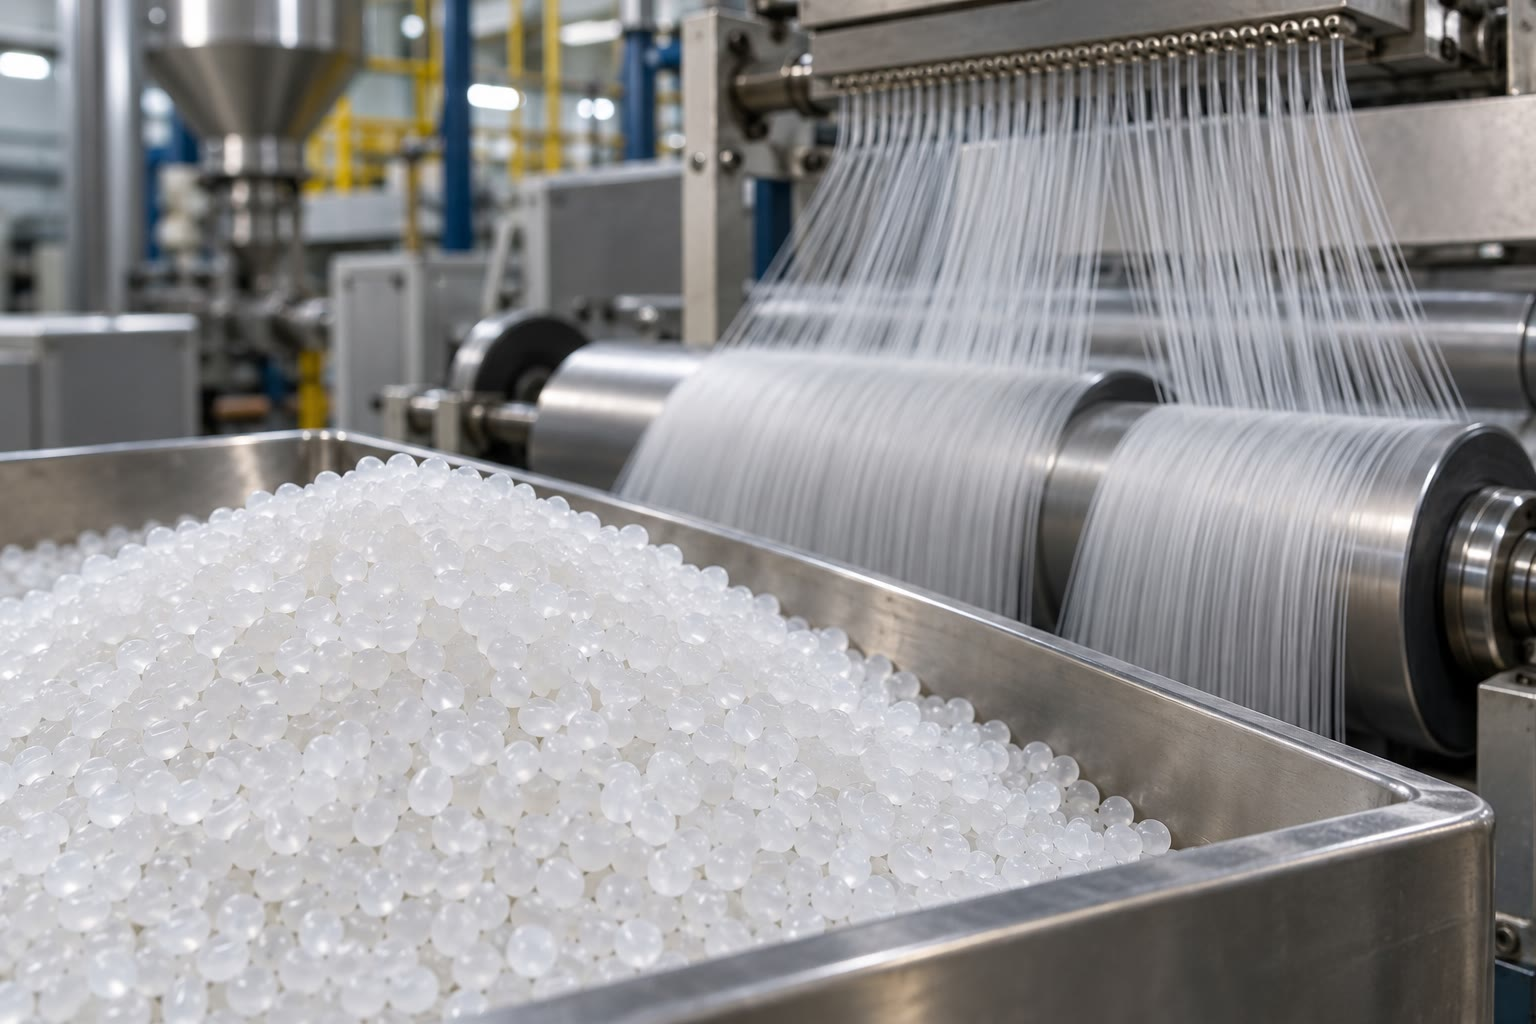
\includegraphics[width=0.58\linewidth]{images/book3/ai/b2-29-pellets.jpg}

{\small حبيبات \omterm{def:b2:polymer-synthesis:polymer}{بوليمر} في مصنع، وهي الهيئة التي تُباع بها اللدائن الحرارية، وألياف تُسحب
من مغزل على بكرات دوّارة خلفها (رسم توضيحي).}
\end{omfigure}

\begin{history}[مردود 99~\% لا يكفي]
\begin{minipage}[t]{0.2\linewidth}
\vspace{0pt}
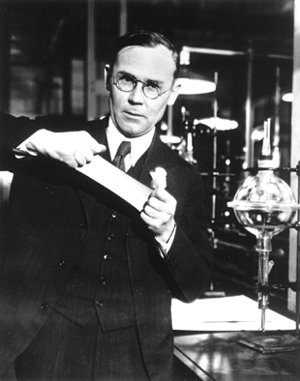
\includegraphics[width=\linewidth]{images/book3/carothers.jpg}
\end{minipage}\hfill
\begin{minipage}[t]{0.76\linewidth}
\vspace{0pt}
والاس كاروثرز، مدرّس جامعي شاب استُقدم إلى مختبر صناعي للبحث
الأساسي، بنى جزيئات طويلة من تفاعلات معروفة، ودعمت نتائجه بقوة
الفكرة التي كانت موضع جدل حينئذ بأن البوليمرات جزيئات عادية، لكنها طويلة جدًا فحسب. وصنع فريقه
البوليسترات، ثم، منذ 1934، البوليأميدات؛ والمعادلة التي تحمل اسمه تفسر لماذا لم تعطِ ألياف إلا
التحويلات القصوى. ودخل النايلون الإنتاج سنة 1939. (صورة: مصور
مجهول، ملكية عامة؛ ويكيميديا كومنز.)
% ledger: hist:polyamides-1934, hist:nylon-production-1939
\end{minipage}
\end{history}

\begin{safety}{\ghs[5mm]{GHS01}\,\ghs[5mm]{GHS02}\,\ghs[5mm]{GHS05}\,\ghs[5mm]{GHS07}\,\ghs[5mm]{GHS08}\,\ghs[5mm]{GHS09}}
الستيرين قابل للاشتعال وخطر على الصحة. وفوق أكسيد ثنائي البنزويل مؤكسد متفجر حين يجف 
ويُحفظ رطبًا وباردًا. والهكسان-1،6-ثنائي الأمين وحمض الهكسانديويك أكّالان للعينين.
% ledger: ghs:styrene, ghs:BPO, ghs:hexanediamine, ghs:adipic-acid
\end{safety}

\section{تمارين}

\begin{exercise}[$\star$]\label{exo:b2:polymer-synthesis:1}
ارسم الوحدات المتكررة للبولي إيثين، والبولي بروبين، والبولي(كلوريد الفينيل)، والبوليستيرين، والنايلون-6،6.
\end{exercise}

\begin{exercise}[$\star$]\label{exo:b2:polymer-synthesis:2}
نمو مرحلي أم سلسلي: PET من الإيثان-1،2-ديول وحمض البنزين-1،4-ثنائي الكربوكسيليك؛ والبوليستيرين؛
والنايلون-6،6؛ والبولي(ميثاكريلات الميثيل)؛ والبولي(حمض اللاكتيك) من حمض 2-هيدروكسي بروبانويك؟
\end{exercise}

\begin{exercise}[$\star$]\label{exo:b2:polymer-synthesis:3}
بوليستيرين له $\bar X_n = 1000$. احسب $\bar M_n$، مع إهمال المجموعات الطرفية.
\end{exercise}

\begin{exercise}[$\star$]\label{exo:b2:polymer-synthesis:4}
سلسلة بولي بروبين مرسومة متعرجة مستوية تقع مجموعات الميثيل فيها في جهة القارئ، ثم
بعيدًا، ثم نحوه، ثم بعيدًا، وهكذا. سمِّ تاكتيكيتها. هل يمكن أن تتبلور؟
\end{exercise}

\begin{exercise}[$\star\star$]\label{exo:b2:polymer-synthesis:5}
عينة هي خليط من كتلتين متساويتين لجزأين، كتلتاهما الموليتان \qty{10}{kg/mol} 
و\qty{100}{kg/mol}. احسب $\bar M_n$ و$\bar M_w$ \omterm{def:b2:polymer-synthesis:averages}{والتشتت}.
\end{exercise}

\begin{exercise}[$\star\star$]\label{exo:b2:polymer-synthesis:6}
احسب $\bar X_n$ لبلمرة متوازنة بالنمو المرحلي عند $p = 0.98$ و$p = 0.995$.
\end{exercise}

\begin{exercise}[$\star\star$]\label{exo:b2:polymer-synthesis:7}
يُخلط ثنائي حمض وثنائي أمين مع فائض 1~\% (بالمولات) من ثنائي الأمين. ما أكبر
$\bar X_n$ يمكن بلوغها؟
\end{exercise}

\begin{exercise}[$\star\star$]\label{exo:b2:polymer-synthesis:8}
في بلمرة جذرية يُضاعَف تركيز البادئ. بأي عامل تتغير سرعة
البلمرة \omterm{def:b2:polymer-synthesis:chain-length}{وطول السلسلة الحركي}؟
\end{exercise}

\begin{exercise}[$\star\star$]\label{exo:b2:polymer-synthesis:9}
البولي(كلوريد الفينيل) صلب؛ وخراطيم الحدائق المصنوعة منه مرنة لأنها تحوي ملدّنًا،
وهو جزيء صغير ممزوج بين السلاسل. فسّر بالتحول الزجاجي.
\end{exercise}

\begin{exercise}[$\star\star\star$]\label{exo:b2:polymer-synthesis:10}
بيّن أن التوزيع الكتلي لفلوري $w_x = x(1-p)^2p^{\,x-1}$، معتبرًا دالة في $x$
متصل، أكبر ما يكون عند $x = -1/\ln p$، وأن هذه القيمة قريبة من $\bar X_n$ حين تكون $p$ قريبة من 1.
\end{exercise}

\begin{exercise}[$\star\star\star$]\label{exo:b2:polymer-synthesis:11}
يُصنع PET على مرحلتين: يعطي البنزين-1،4-ثنائي الكربوكسيلات ثنائي الميثيل مع فائض من الإيثان-1،2-ديول
البنزين-1،4-ثنائي الكربوكسيلات ثنائي(2-هيدروكسي إيثيل) والميثانول؛ ثم يُسخَّن هذا الإستر الثنائي تحت التخلية
فيتبلمر، مطلقًا الإيثان-1،2-ديول. اكتب المرحلتين وفسّر كيف تحل المرحلة الثانية
مشكلة قياسات الكميات في معادلة كاروثرز.
\end{exercise}

\begin{exercise}[$\star\star\star$]\label{exo:b2:polymer-synthesis:12}
في بلمرة جذرية مشتركة للمونومرين 1 و2، يُعطى التركيب اللحظي \omterm{def:b2:polymer-synthesis:copolymer}{للبوليمر المشترك}
بالعلاقة $\dfrac{\mathrm d[\mathrm M_1]}{\mathrm d[\mathrm M_2]} = \dfrac{[\mathrm M_1](r_1[\mathrm M_1]
+ [\mathrm M_2])}{[\mathrm M_2]([\mathrm M_1] + r_2[\mathrm M_2])}$، حيث $r_1$ و$r_2$
نسبتا التفاعلية (معطيات التمرين: $r_1 = 2.0$، $r_2 = 0.5$). احسب نسبة الوحدات في
\omterm{def:b2:polymer-synthesis:copolymer}{البوليمر المشترك} المتكوّن من تغذية متساوية المولات. ماذا يحدث إذا كان $r_1 = r_2 = 0$؟
\end{exercise}

\section{مسألة: النايلون-6،6 بالكيلوغرام}

\begin{problem}[{مسألة نهاية الأسبوع --- المونومران وملح النايلون، ومعادلة كاروثرز، 
وعدم توازن مقصود، وتوزيع فلوري والماء المتحرر}]
\label{pb:b2:polymer-synthesis:1}
يُصنع النايلون-6،6 من الهكسان-1،6-ثنائي الأمين وحمض الهكسانديويك. وتُهمل المجموعات الطرفية في كل المسألة.
والكتل المولية (\unit{g/mol}): C 12.011، H 1.008، N 14.007، O 15.999.
% ledger: aw:C, aw:H, aw:N, aw:O, ghs:hexanediamine, ghs:adipic-acid

\medskip
\noindent\textbf{الجزء الأول --- المونومران \omterm{def:b2:polymer-synthesis:polymer}{والوحدة المتكررة}.}
\begin{enumerate}
  \item اكتب صيغتي المونومرين.
  \item اكتب معادلة تكوّن رابطة أميد واحدة.
  \item يُجمع المونومران أولًا على هيئة ملح 1\,:\,1، يُبلور من المحلول. لماذا؟
  \item أعطِ \omterm{def:b2:polymer-synthesis:polymer}{الوحدة المتكررة} للنايلون-6،6، وصيغتها وكتلتها المولية.
  \item ما الكتلة المولية المتوسطة $M_0$ لوحدة مشتقة من \omterm{def:b2:polymer-synthesis:polymer}{مونومر} في السلسلة؟
  \item ماذا يعدّ الرقمان في الاسم «6،6»؟
\end{enumerate}

\medskip
\noindent\textbf{الجزء الثاني --- معادلة كاروثرز.}
\begin{enumerate}[resume]
  \item احسب $\bar X_n$ و$\bar M_n$ عند $p = 0.98$.
  \item السؤال نفسه عند $p = 0.99$.
  \item فسّر الملاحظة «مردود 99~\% لا يكفي».
  \item أي درجة تقدم تعطي $\bar M_n = \qty{10}{kg/mol}$؟
  \item كيف تُدفع درجة التقدم إلى هذا الارتفاع عمليًا؟
  \item لماذا يجب أن يكون المونومران نقيين جدًا؟
\end{enumerate}

\medskip
\noindent\textbf{الجزء الثالث --- عدم توازن مقصود.}
\begin{enumerate}[resume]
  \item يُستعمل ثنائي الأمين بفائض مولي قدره 1~\%. احسب $r$.
  \item احسب أكبر $\bar X_n$ و$\bar M_n$ يمكن بلوغهما حينئذ.
  \item احسب $\bar X_n$ عند $p = 0.99$ مع عدم التوازن هذا.
  \item أي المجموعات تنهي السلاسل في نهاية التفاعل؟
  \item يُضاف أحيانًا قليل من حمض الإيثانويك. ماذا يفعل بالسلاسل؟
  \item لماذا يحد المصنِّع طول السلاسل عن قصد؟
\end{enumerate}

\medskip
\noindent\textbf{الجزء الرابع --- التوزيع والموازنة الكتلية.}
\begin{enumerate}[resume]
  \item من أجل خليط متوازن عند $p = 0.99$، أعطِ \omterm{def:b2:polymer-synthesis:averages}{التشتت}.
  \item احسب $\bar M_w$ عند $p = 0.99$.
  \item عند $p = 0.99$، ما كسر الجزيئات، وما كسر الكتلة، الذي ما زال مونومرًا
        لم يتفاعل؟
  \item قرب أي طول سلسلة يكون التوزيع الكتلي أكبر ما يمكن؟
  \item احسب كتلة الماء المتحرر لكل كيلوغرام من النايلون-6،6.
  \item لماذا يتطلب الغزل بالصهر $\bar M_n$ ضمن نافذة محددة؟
  \item اذكر درجة التقدم التي تعطي $\bar M_n = \qty{20}{kg/mol}$ لخليط متوازن.
\end{enumerate}
\end{problem}
